\documentclass{article}
\usepackage{polski} %moze wymagac dokonfigurowania latexa, ale jest lepszy niż standardowy babel'owy [polish] 
\usepackage[utf8]{inputenc} 
\usepackage[OT4]{fontenc} 
\usepackage{graphicx,color} %include pdf's (and png's for raster graphics... avoid raster graphics!) 
\usepackage{url} 
%\usepackage{cite}
\usepackage{biblatex}
\usepackage[pdftex,hyperfootnotes=true,pdfborder={0 0 0}]{hyperref} %za wszystkimi pakietami; pdfborder nie wszedzie tak samo zaimplementowane bo specyfikacja nieprecyzyjna; pod miktex'em po prostu nie widac wtedy ramek
\bibliography{sprawozdanie}

% Zmiana rozmiar�w strony tekstu
\addtolength{\voffset}{-1cm}
\addtolength{\hoffset}{-1cm}
\addtolength{\textwidth}{2cm}
\addtolength{\textheight}{2cm}

%bardziej zyciowe parametry sterujace rozmieszczeniem rysunkow
\renewcommand{\topfraction}{.85}
\renewcommand{\bottomfraction}{.7}
\renewcommand{\textfraction}{.15}
\renewcommand{\floatpagefraction}{.66}
\renewcommand{\dbltopfraction}{.66}
\renewcommand{\dblfloatpagefraction}{.66}
\setcounter{topnumber}{9}
\setcounter{bottomnumber}{9}
\setcounter{totalnumber}{20}
\setcounter{dbltopnumber}{9}

% w�asny bullet list z malymi odstepami
\newenvironment{tightlist}{
\begin{itemize}
  \setlength{\itemsep}{1pt}
  \setlength{\parskip}{0pt}
  \setlength{\parsep}{0pt}}
{\end{itemize}}




\begin{document}

\thispagestyle{empty} %bez numeru strony

\begin{center}
{\large{Sprawozdanie II z laboratorium:\\
Uczenie Maszynowe i Sieci Neuronowe}}

\vspace{3ex}

Część I: Uczenie nadzorowane warstwowych sieci neuronowych

Część II: Rekurencyjne sieci neuronowe

Część III: Uczenie nienadzorowane warstwowych sieci neuronowych


\vspace{3ex}
{\footnotesize\today}

\end{center}


\vspace{10ex}

Prowadzący: dr inż. Maciej Komosiński

\vspace{5ex}

Autorzy:
\begin{tabular}{lllr}
\textbf{Krzysztof Urban} & inf84896 & ISWD & krz.urb@gmail.com \\
\textbf{Tomasz Ziętkiewicz} & inf84914 & ISWD & tomek.zietkiewicz@gmail.com \\
\end{tabular}

\vspace{5ex}

Zajęcia poniedziałkowe; Krzysztof: 16:50, Tomasz: 13:30

\newpage



%%%%%%%%%%%%%%%%%% Część I %%%%%%%%%%%%%%%%%

\section{Uczenie nadzorowane warstwowych sieci neuronowych}

\subsection{Różnice funkcjonalne pomiędzy sieciami jedno- i wielowarstwowymi oraz pomiędzy sieciami liniowymi a nieliniowymi (uczenie sieci warstwowych funkcji logicznej AND i funkcji różnicy symetrycznej XOR)}

\begin{enumerate}
\item \textbf{
Skonstruuj zbiór przykładów definiujący dwuargumentową funkcję ("bramkę") AND (File|New|Data set) i zachowaj go. Wszystkie 4 przykłady mają stanowić zbiór uczący. Jakie są klasy decyzyjne w tym zbiorze przykładów i jakie są ich liczności?}
\begin{figure}[h]
\centering
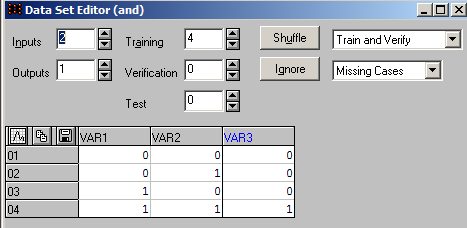
\includegraphics[scale=0.75]{dane/part1/zad2/dataset_and}
\caption{Zbiór uczący funkcji "AND"\label{fig:dataset_and}}
\end{figure}

\item \textbf{
Wyszukaj w Pomocy hasło "Verification" i przeczytaj wszystkie pięć znalezionych tematów.}

\item \textbf{
Wyobraź sobie (narysuj) pożądaną funkcję odpowiedzi sieci (trójwymiarowy wykres zależności wyjścia od dwóch wejść).}

\item \textbf{
Skonstruuj liniową sieć jednowarstwową o architekturze 2-1 (File|New|Network, Type=Linear, przycisk Advise). Uaktywnij okno wykresu błędu średniokwadratowego (Statistics|Training graph). Naucz sieć na problemie AND (Train|Multilayer perceptron|Back propagation). Obejrzyj funkcję odpowiedzi sieci (Run|Responce surface) i błędy dla poszczególnych przypadków (Statistics|Case errors).}
 
\begin{figure}[h]
\centering
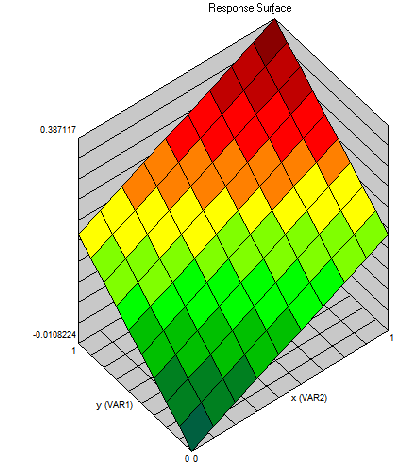
\includegraphics[scale=0.75]{dane/part1/zad2/response}
\caption{Funkcja odpowiedzi sieci liniowej. Problem "AND".\label{fig:response_linear}}
\end{figure}

\begin{figure}[h]
\centering
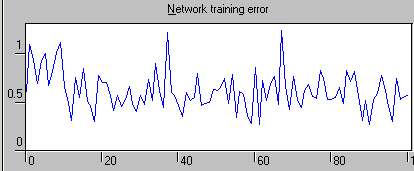
\includegraphics[width=0.6\textwidth]{dane/part1/zad2/error}
\caption{Błąd średniokwadratowy dla sieci liniowej. Problem "AND".\label{fig:error_linear}}
\end{figure}
%
%\begin{figure}[h]
%\centering
%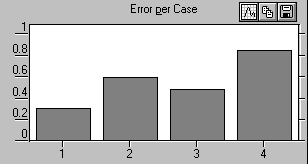
\includegraphics[width=0.6\textwidth]{dane/part1/zad2/error_case}
%\label{fig:error_linear_case}
%\caption{Błąd dla poszczególnych przypadków dla sieci liniowej. Problem "AND".}
%\end{figure}

Funkcję odpowiedzi sieci i błąd przez nią popełniany pokazano na rys. \ref{fig:response_linear} i \ref{fig:error_linear}. Sieć nie radzi sobie z zadaniem - przez swą liniową naturę zawsze średnia wartość funkcji w punktach (0,1) i (1,0)  będzie równa średniej wartości w punktach (0,0) i (1,1) przez co wagi mogą jedynie zmienić rozłożenie błędu między poszczególne przypadki uczące, ale zawsze zmniejszanine błędu w punktach (0,0), (0,1) i (1,0) będzie powodowało wzrost błędu w punkcie (1,1) i na odwrót. Przy zmniejszeniu prędkości uczenia błąd sieci można zredukować do ok 0.2.

\item \textbf{
Spróbuj utworzyć sieć liniową dla problemu AND o liczbie warstw większej niż 2.}
\\Porgram nie pozwala na utworzenie takiej sieci, ponieważ nie ma to sensu - po dodaniu dodatkowych warstw końcowa funkcja aktywacji będzie tylko kombinacją liniową funkcji poszczególnych neuronów. Dodatkowe warstwy są redundantne, ponieważ dla każdej liniowej sieci 3 i więcej warstwowej istnieje odpowiadająca jej sieć 2 warstwowa, której zachowanie jest identyczne.

\item \textbf{
Przerób sieć na nieliniową sieć jednowarstwową (ustawiając Act fn w Edit|Network na Logistic) i naucz ją na tym samym problemie.}

\begin{figure}[h]
\centering
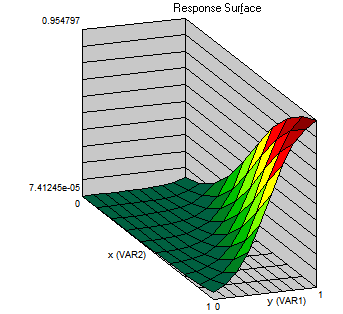
\includegraphics[scale=1.0]{dane/part1/zad2/response_nonlinear}
\caption{Funkcja odpowiedzi sieci nieliniowej jednowarstwowej. Problem "AND".\label{fig:response_nonlinear}}
\end{figure}

\begin{figure}[h]
\centering
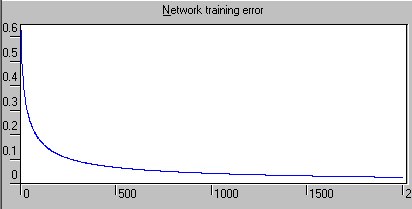
\includegraphics[width=0.6\textwidth]{dane/part1/zad2/error_nonlinear}
\caption{Błąd średniokwadratowy dla sieci nieliniowej jednowarstwowej. Problem "AND".\label{fig:error_nonlinear}}
\end{figure}

\begin{figure}[h]
\centering
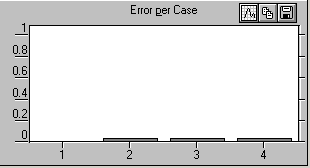
\includegraphics[width=0.6\textwidth]{dane/part1/zad2/error_case_nonlinear}
\caption{Błąd dla poszczególnych przypadków dla sieci nieliniowej jednowarstwowej. Problem "AND".\label{fig:error_nonlinear_case}}
\end{figure}

Sieć nielinowa poradziła sobie z problemem znacznie lepiej - błędy klasyfikacji bliskie zeru. W przeciwieństwie do sieci liniowej proces uczenia jest zbieżny - wraz z uczeniem błąd asymptotycznie maleje. Widać to na rysunku \ref{fig:error_nonlinear}.

\item \textbf{
Wejdź do edytora sieci (Network|Edit) i przypatrz się wagom neuronu wyjściowego. Wykreśl w przestrzeni wejść prostą, którą definiuje neuron wyjściowy i oceń, czy i jak realizuje ona separację klas decyzyjnych. }
\begin{figure}[h]
\centering
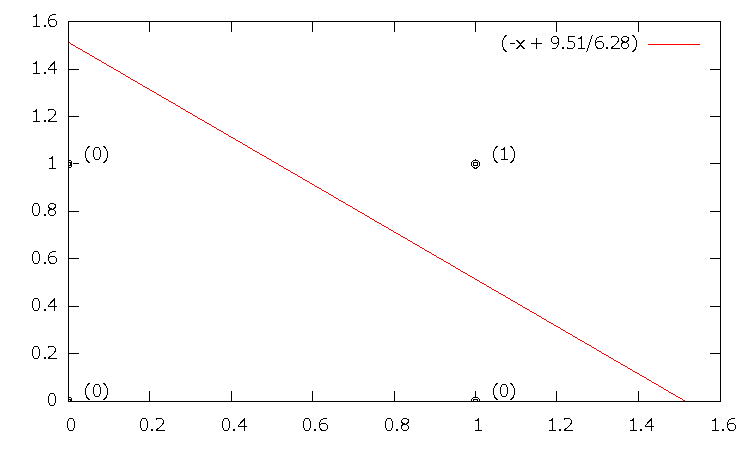
\includegraphics[width=0.8\textwidth]{dane/part1/zad2/separacja_and}
\caption{Prosta separująca klasy decyzyjne dla problemu "AND".\label{fig:prosta_separujaca}}
\end{figure}
\\Prosta ta jest przedstawiona na rys. \ref{fig:prosta_separujaca}. Separuje ona prawidłowo punkty należące do klas 0 i 1. Jeśli za kryterium oceny separacji uznać maksymalizację minimalnej odleglości prostej od separowanych punktów, to trzeba uznać, że realizuje ją dobrze, ponieważ odległość ta jest taka sama dla punktów (0,1), (1,0) i (1,1). Zmiana jakichkolwiek parametrów prostej, po której prosta ta wciąż separowałaby klasy, wiązałaby się ze zmniejszeniem minimalnej odległości punktów od prostej, więc ze względu na to kryterium prosta separująca jest optymalna.

\item \textbf{
Skonstruuj zbiór przykładów definiujący dwuargumentową funkcję XOR i zachowaj go. Wszystkie 4 przykłady mają stanowić zbiór uczący.}
\begin{figure}[h]
\centering
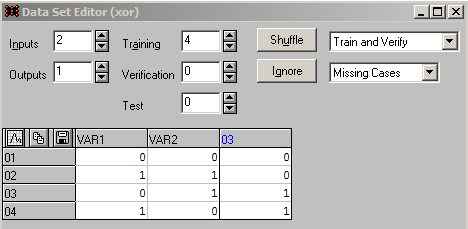
\includegraphics[scale=0.75]{dane/part1/zad2/dataset_xor}
\caption{Zbiór uczący funkcji "XOR"\label{fig:dataset_xor}}
\end{figure}
\\Zbiór uczący dla funkcji XOR pokazano na rys. \ref{fig:dataset_xor}. 

\item \textbf{
Wyobraź sobie (narysuj) pożądaną funkcję odpowiedzi sieci.}

\item \textbf{
Skonstruuj liniową sieć jednowarstwową o architekturze 2-1 i naucz ją na problemie XOR.}

\item \textbf{ Obejrzyj funkcję odpowiedzi sieci i błędy dla poszczególnych przypadków.}
\begin{figure}[h]
\centering
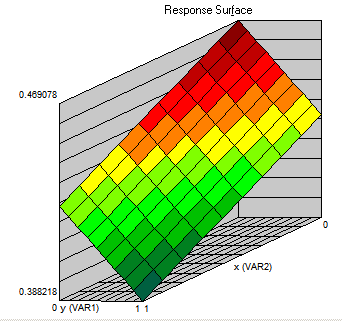
\includegraphics[scale=0.75]{dane/part1/zad2/response_xor}
\caption{Funkcja odpowiedzi sieci liniowej dla problemu "XOR"\label{fig:response_linear_xor}}
\end{figure}

\begin{figure}[h]
\centering
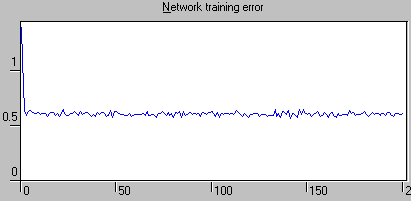
\includegraphics[width=0.6\textwidth]{dane/part1/zad2/error_xor}
\caption{Błąd średniokwadratowy sieci liniowej dla problemu "XOR".\label{fig:error_linear_xor}}
\end{figure}

\begin{figure}[h]
\centering
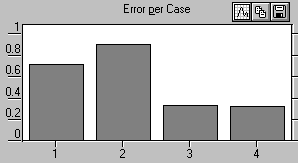
\includegraphics[width=0.6\textwidth]{dane/part1/zad2/error_case_xor}
\caption{Błąd sieci liniowej dla problemu "XOR" dla poszczególnych przypadków .\label{fig:error_case_linear_xor}}
\end{figure}

Jak widać na rysunkach \ref{fig:response_linear_xor}, \ref{fig:error_linear_xor} i \ref{fig:error_case_linear_xor} sieć liniowa nie radzi sobie z zadaniem.



\item \textbf{
Przerób sieć na nieliniową sieć jednowarstwową i naucz ją na tym samym problemie (zwróć uwagę, jak sieć stara się minimalizować błąd). Obejrzyj, jak zmienia się rozkład wag podczas procesu uczenia (Statistics|Weight distribution).}
\\Błąd średniokwadratowy i funkcję odpowiedzi sieci nieliniowej jednowarstwowej dla problemu "XOR" przedstawiono na rysunkach \ref{fig:error_nonlinear_xor} i \ref{fig:response_nonlinear_xor}.

\begin{figure}[h]
\centering
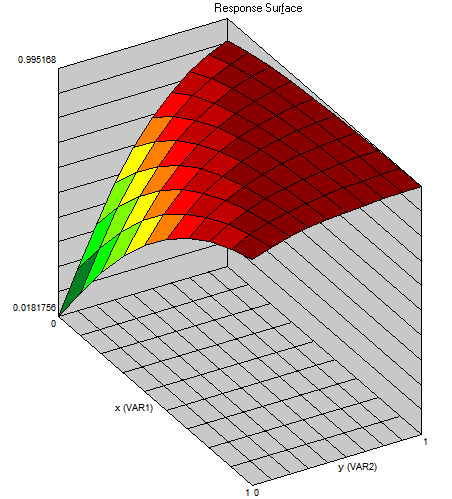
\includegraphics[scale=0.75]{dane/part1/zad2/response_nonlinear_xor}
\caption{Funkcja odpowiedzi sieci nieliniowej jednowarstwowej dla problemu "XOR".\label{fig:response_nonlinear_xor}}
\end{figure}

\begin{figure}[h]
\centering
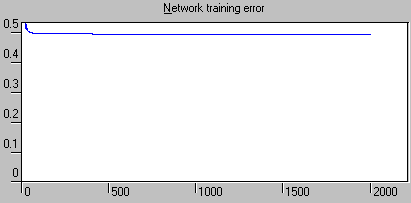
\includegraphics[width=0.6\textwidth]{dane/part1/zad2/error_nonlinear_xor}
\caption{Błąd średniokwadratowy sieci nieliniowej jednowarstwowej dla problemu "XOR".\label{fig:error_nonlinear_xor}}
\end{figure}

\item \textbf{
Skonstruuj nieliniową sieć dwuwarstwową o architekturze 2-2-1 (File|New|Network, Type=Multilayer perceptron) i naucz ją na problemie XOR. Obejrzyj funkcję odpowiedzi.}
\\Funkcję odpowiedzi i błąd średniokwadratowy przedstawiono na rys. \ref{fig:response_221_xor} i \ref{fig:error_221_xor}
\begin{figure}[h]
\centering
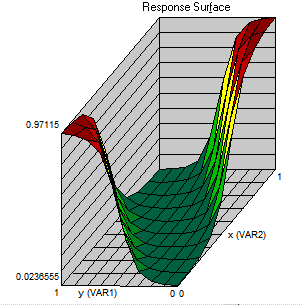
\includegraphics[scale=0.75]{dane/part1/zad2/response_221_xor}
\caption{Funkcja odpowiedzi sieci nieliniowej 2-2-1 dla problemu "XOR".\label{fig:response_221_xor}}
\end{figure}

\begin{figure}[h]
\centering
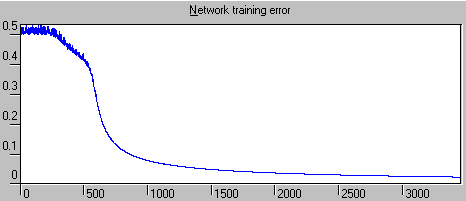
\includegraphics[width=0.6\textwidth]{dane/part1/zad2/error_221_xor}
\caption{Błąd średniokwadratowy sieci nieliniowej 2-2-1 dla problemu "XOR"..\label{fig:error_221_xor}}
\end{figure}


\item \textbf{
Obejrzyj wagi sieci w edytorze sieci (Edit|Network). Jakie proste definiują neurony w warstwie ukrytej (spróbuj je narysować w przestrzeni wejść) ? Jak można interpretować działanie neuronu wyjściowego ?}
\\Proste definiowane przez neurony w warstwie ukrytej pokazano na rys. \ref{fig:prosta_separujaca_xor}. Ponieważ wagi neuronu wyjściowego są zbliżone do wartości progu tego neuronu, to jego działanie można interpretować jako sumę logiczną: jeśli na jednym z wejść wartość jest bliska 1 lub większa, to na wyjściu neuronu wyjściowego również wartość będzie zbliżona do 1. Dzięki temu akumulowane są wyniki działania neuronów z warstwy ukrytej i zarówno dla wartości wejściowych (0,1) jak i (1,0) sieć daje prawidłową odpowiedź: 1.

\begin{figure}[h]
\centering
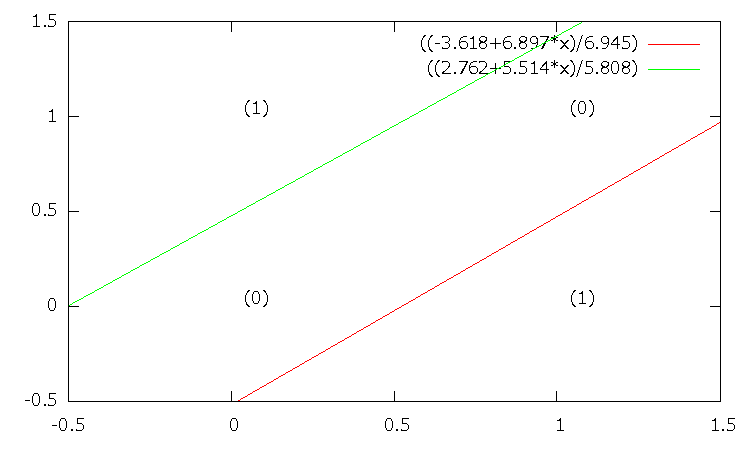
\includegraphics[width=0.8\textwidth]{dane/part1/zad2/separacja_xor_ukryta}
\caption{Proste separująca klasy decyzyjne dla problemu "XOR". Neurony warstwy ukrytej.\label{fig:prosta_separujaca_xor}}
\end{figure}


\item \textbf{
Obejrzyj, jak zmienia się rozkład wag podczas procesu uczenia. Jaka jest przyczyna takiego zachowania wag i jakie to może mieć konsekwencje (z "informatycznego" punktu widzenia) ?}
\\Na początku wagi zbliżają się do bardzo małyych wartości bliskich zeru, co może doprowadzić do tego, że z powodu skończonej precyzji zapisu liczb rzeczywistych zostaną one wyzerowane.

\end{enumerate}

\subsection{Obserwacja zjawiska przeuczenia na przykładzie zbioru PIMA.}
\begin{enumerate}
\item \textbf{ Zapoznaj się z pochodzeniem zbiorów PIMA i BUPA (wyszukaj: "PIMA dataset", "BUPA dataset").}
\\Zbiór PIMA zawiera dane dotyczące cukrzycy wśród indian Pima. Jest to zbiór o charakterze diagnostycznym: zawiera ogólne dane medyczne (8 atrbutów) i jeden bnarny atrybut decyzyjny (chory/zdrowy). Zbiór zawiera ukryte brakujące dane (nierzeczywiste wartości pewnych parametrów, np. ciśnienie krwi równe 0 )
\\Zbiór BUPA zawiera wyniki testów krwi które mogą wskazywać choroby wątroby, atrybut określający ilość sporzywanego dziennie alkoholu oraz jeden atrybut decyzyjny. Zbiór nie posiada brakujących wartości.

\item \textbf{
Wczytaj zbiór PIMA i skonstruuj dla niego dwuwarstwową sieć nieliniową o architekturze 8-4-1.}

\item \textbf{
Obejrzyj ustawienia w okienku Pre/Post Processing.}

\item \textbf{
Wyłącz "inkrementacyjne" warunki stopu ustawiając np. zero lub dużą wartość parametru Window w oknie Stopping Conditions.}

\item \textbf{
Przeprowadź uczenie algorytmem wstecznej propagacji błędu (może być bardzo długie, np. 20 000 epok); obserwuj przebieg błędu dla zbioru uczącego i weryfikującego.}
\end{enumerate}

\subsection{Dobór liczby neuronów w warstwie ukrytej na przykładzie zbioru IRIS.}
\begin{enumerate}
\item \textbf{ Dla zbioru IRIS przeprowadź co najmniej 5 eksperymentów uczenia nieliniowych sieci dwuwarstwowych o architekturach 4-n-3, dla n zmieniającego się w przedziale [2,10], przy wyłączonym kryterium warunku stopu na zbiorze weryfikacyjnym. Po każdym eksperymencie kopiuj przebieg błędu przez schowek do Notatnika.}

\item \textbf{
Przedstaw w gnuplocie na jednym wykresie przebieg błędu uczenia dla kolejnych wartości n.}

\item \textbf{
Czy istnieje jednoznaczna zależność pomiędzy n a przebiegiem błędu średniokwadratowego? Czy biorąc pod uwagę tylko przebeg błędu dla zbioru uczącego można ustalić optymalną liczbę neuronów w warstwie ukrytej? Jeśli tak, to ile ona wynosi dla tego zbioru przykładów?}
\end{enumerate}

\subsection{Sterowanie rozmiarem obszaru niepewnych odpowiedzi (braku odpowiedzi) sieci na granicach klas decyzyjnych (podczas testowania sieci)}
\begin{enumerate}
\item \textbf{Utwórz i naucz sieć na zbiorze PIMA (architektura 8-4-1).}

\item \textbf{
Przeprowadź klasyfikowanie przykładów ze zbioru testującego (okno Statistics|Classification). Znajdź w tym oknie macierz pomyłek (ang. confusion matrix).}

\item \textbf{
Otwórz okno Edit|Pre-Post Processing. Pola Accept i Reject definiują, jakie wartości muszą mieć neurony w warstwie wyjściowej, aby móc zinterpretować ich stan jako decyzję o przypisaniu przykładu do odpowiedniej klasy decyzyjnej. Choć nie jest to kontrolowane przez program, powinno zachodzić Accept >= Reject}

\item \textbf{
Przy użyciu gnuplota sporządź wykres (trzy przebiegi na jednym wykresie) zależności procentu przypadków z jednego ze zbiorów (uczącego / weryfikującego / testującego):
– poprawnie zaklasyfikowanych (do wszystkich klas decyzyjnych razem),
– niepoprawnie zaklasyfikowanych,
– niezaklasyfikowanych
w funkcji progu Accept, dla następujących wartości Accept i Reject:
\begin{tabular}{|c|c|}
\hline Accept & Reject \\ 
\hline 0.5 & 0.5 \\ 
\hline 0.6 & 0.4 \\ 
\hline 0.7 & 0.3 \\ 
\hline 0.8 & 0.2 \\ 
\hline 0.9 & 0.1 \\ 
\hline 1.0 & 0.0 \\ 
\hline 
\end{tabular} 
}

\item \textbf{
Czy na podstawie otrzymanego wykresu można zasugerować jakąś optymalną wartość obu progów dla tego zbioru przykładów i tej sieci?}

\end{enumerate}

\subsection{Badanie odporności sieci na uszkodzenia}
\begin{enumerate}
\item \textbf{Skonstruuj sieć dwuwarstwową o architekturze 4-3-3 dla problemu IRIS i naucz ją.}

\item \textbf{
Przeprowadź testowanie i zapisz trafność klasyfikowania.}

\item \textbf{
Otwórz edytor sieci (Edit|Network). Wyszukaj (w obu warstwach: ukrytej i wyjściowej!) i usuń z sieci (tj. wyzeruj) wagę najmniejszą co do wartości bezwzględnej (pomiń wiersz Threshold, zawierający progi neuronów). Przeprowadź ponownie testowanie sieci i zapisz wynik.}

\item \textbf{
Kroki z punku 3 powtórz ok. 10 razy, kolejno usuwając coraz większe wagi i notując trafność klasyfikowania. Sporządź wykres zależności trafności klasyfikowania w funkcji ilości usuniętych (najmniejszych) wag.}

\item \textbf{
Czy odporność sieci na uszkodzenia (usunięcia wag) jest wysoka?}

\item \textbf{
Czy jesteś w stanie na podstawie tak “zredukowanej” sieci powiedzieć coś o ważności poszczególnych atrybutów opisujących przykłady?}

\item \textbf{
Czy w konsekwencji “przerzedzenia” sieci można usunąć niektóre neurony? Jak należy to zrobić? (przemyśl dokładnie).}
\end{enumerate}

\subsection{ Eksperymentalny dobór rozmiaru zbioru weryfikującego}
Dla zbioru IRIS, PIMA lub BUPA przeprowadź eksperyment uczenia i testowania, zmieniając proporcje pomiędzy zbiorem uczącym i weryfikującym.
\begin{enumerate}
\item \textbf{Zacznij od następujących proporcji zbioru uczącego, weryfikującego i testującego 8:1:1.}

\item \textbf{
Przeprowadź uczenie (liczba epok >=300). Przetestuj sieć, zapisz trafność klasyfikowania, błąd klasyfikowania i procent przykładów niezaklasyfikowanych.}

\item \textbf{
Sukcesywnie zwiększaj rozmiar zbioru weryfikującego, zmniejszając rozmiar uczącego (pole Training w oknie Edit|Data set), do proporcji 1:8:1 włącznie.}

\item \textbf{
Sporządź wykres zależności trafności klasyfikowania, błędu klasyfikowania i procentu przykładów niezaklasyfikowanych w funkcji proporcji rozmiaru zbioru weryfikującego do liczby przykładów, jakie mamy do dyspozycji podczas uczenia (czyli rozmiar zbioru uczącego + rozmiar zbioru weryfikującego). Czy można znaleźć jakąś wielkość optymalną?
}
\end{enumerate}

\subsection{Porównanie ‘vanilla’ backpropagation z bardziej wyrafinowanymi algorytmami uczenia nadzorowanego sieci warstwowych}
\textbf{Dla zbioru PIMA lub BUPA przeprowadź eksperyment uczenia i testowania, używając poza standardowym (vanilla) algorytmem backpropagation innych algorytmów uczenia (np. QuickPropagation, Delta-bar-Delta). Dla zapewnienia porównywalności wyników, w poszczególnych eksperymentach zachowaj tą samą konfigurację sieci i warunki stopu. W miarę możliwości uśrednij wyniki z kilku przebiegów dla każdego algorytmu. Czy któryś z algorytmów jest wyraźnie lepszy? Porównaj liczbę epok uczenia.
\\
Uwaga. Algorytmy QuickProp i DeltaBarDelta mogą okazać się trochę niestabilne (w ogólności łatwiej niż backprop wpadają w minima lokalne). W takim przypadku trzeba się trochę pobawić parametrami.}

\subsection{Inne sieci warstwowe – sieci z jednostkami o symetrii kołowej (RBF)}
\begin{enumerate}
\item \textbf{Zbuduj sieć RBF dla problemu IRIS.
Otwórz edytor sieci (Edit|Network). Zwróć uwagę na różnice w polach Act fn i PSP in w porównaniu z perceptronami.}

\item \textbf{
Naucz sieć. Uczenie składa się z trzech etapów: ustalania centrów poszczególnych neuronów, ustalenia promieni (deviation), które decydują o stopniu “spłaszczenia” funkcji Gaussowskich, oraz obliczenia wag neuronu wyjściowego. Zwróć uwagę na czas uczenia.}

\item \textbf{
Obejrzyj funkcję odpowiedzi wybranych neuronów w warstwie ukrytej i neuronów w warstwie wyjściowej (Run|Response Surface). Możesz zmieniać też zmienne niezależne (atrybuty). Zauważ różnice w stosunku do sieci z jednostkami logistycznymi.}

\item \textbf{
Zastanów się, jakie konsekwencje ma niewłaściwy dobór promieni. Co będzie się działo, gdy promienie będą za duże? Co, gdy za małe? (związek z generalizacją).}

\item \textbf{
Przetestuj sieć dla różnych metod uczenia, tj. dla różnych inicjalizacji centrów (Sample, K-means) i różnych sposobów ustalania odchyleń (Explicit, Isotropic, K-nearest). Najlepiej miej otwarty edytor sieci; obserwuj jakie konsekwencje ma wybranie poszczególnych sposobów uczenia.}

\item \textbf{
Porównaj sieć RBF z siecią typu Multilayer Perceptron na trudniejszym zbiorze przykładów (PIMA lub BUPA).}
\end{enumerate}

\subsection{ Uzyskiwanie jak najwyższej trafności}
Manipulując:
\begin{itemize}
\item \textbf{architekturą sieci,}
\item \textbf{prędkością uczenia (można zmieniać dynamicznie),}
\item \textbf{zakresem wartości używanych do inicjalizacji wag sieci,}
\item \textbf{warunkami stopu (statycznymi i/lub dynamicznymi),}
\item \textbf{rodzajem algorytmów,}
\end{itemize}
spróbuj uzyskać jak największą trafność klasyfikowania na zbiorze testującym dla zbioru PIMA lub BUPA.
\\Jeśli możesz, porównaj uzyskany wynik z trafnością otrzymaną przy użyciu drzew decyzyjnych.
\\Aby zapewnić porównywalność wyników i powtarzalność eksperymentu, nie zmieniaj oryginalnego przyporządkowania przykładów do zbiorów uczącego, weryfikującego i testującego.

%%%%%%%%%%%%%%%%%% Część II %%%%%%%%%%%%%%%%%

\section{Rekurencyjne sieci neuronowe}

\subsection{ Kodowanie sieci neuronowych o dowolnej topologii}

\begin{itemize}
\item \textbf{
Napisz w dowolnym języku/narzędziu sparametryzowany generator warstwowych-sieci-feed-forward albo każdy-z-każdym dla f0 lub f1.}	

\begin{lstlisting}[language=python]
from random import random
import sys
'''
Simple NN generator 
Given number of neurons in each layer it generates feed-forward network in f1 notation, with random weights.
First layer is input layer: number of neurons in the first layer is equal to number of inputs of the network.
'''
def generate(neuron_type, layers):        
    print"""org:
name: Anonymous framstick
genotype:~"""
    genotype = "X"
    inputs_no = 0  
    for layer, layer_size in enumerate(layers):
        if(layer > 0):
            inputs_no = layers[layer - 1]
        first_input = 1
        for neuron in range(layer_size):
            genotype += "[%s" % (neuron_type, )
            for input_neuron in range(first_input, first_input + inputs_no):
                weight = random()
                genotype += ", %d:%f" % (-input_neuron, weight)
            genotype += "]"
            first_input +=  1
    print genotype
    print "~\n"
            

if __name__ == '__main__':
    if sys.argv[1] == '-h' or sys.argv[1] == '--help':
        print """
        Simple NN generator 
        Given number of neurons in each layer it generates
        feed-forward network in f1 notation, with random weights.
        
        usage:
            nn_generator.py N a b c
        where:
            N - number of genotypes to generate
            a - number of neurons in first layer
            b - number of neurons in second layer
            c - ...
         example:
            nn_generator.py 5 3 4 1
         will generate 5 genotypes, each with neural network of architecture 3-4-3."""
    else:
        N = int(sys.argv[1])
        layers = [int(c) for c in sys.argv[2:]]
        neuron_type = "Nu"
        for i in range(0,N):
            generate(neuron_type, layers)
\end{lstlisting}

\end{itemize}

\subsection{ Optymalizacja wag i topologii }

\begin{enumerate}
\item \textbf{Mutacja.}
	\begin{itemize}
		\item Ustaw parametry mutacji (Experiment->Genetics) w f0 i f1 tak, żeby dotyczyły tylko dodawania/usuwania neuronów i dodawania/usuwania połączeń. Ustaw "Neurons to add" na jeden rodzaj neuronu – Nu.
		\item Stwórz kilkanaście razy sekwencję 200 mutantów zaczynając od sieci z jednym neuronem. Co można powiedzieć o tych sekwencjach? Pomocniczo zrób wykresy liczby neuronów i połączeń neuronowych w funkcji n. 
W konsoli:
		\begin{verbatim}
		//make mutant sequence.
//ensure there is one genotype in the gene pool! 
var n,ile=200;
GenePools.group=0; //select first group
for(n=1;n<=ile;n++)
{
   GenePools.genotype=n-1; //select n-th genotype as ancestor
   GenePools.mutateSelected();
   Genotype.name="mutant "+n; //set its name to consecutive number
   GenePools.copySelected(0);
   //Simulator.print(""+n+" "+Genotype.nnsiz);
}
		\end{verbatim}

Na rysunkach \ref{fig:mutations-neurons} oraz \ref{fig:mutations-connections} pokazano odpowiednio ilość neuronów i ilość połączeń między nimi w funkcji ilość mutacji. Widać na nich, że w trakcie mutacji neurony i połączenia między nimi są zarówno dodawane jak i odejmowane, sama mutacja bez presji selekcyjnej nie prowadzi w żadnym kierunku.
		
	\begin{figure}[h]
	\centering
	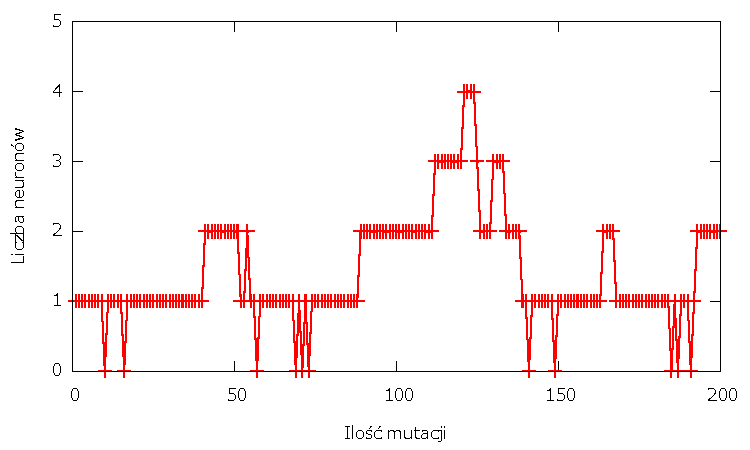
\includegraphics[width=0.8\textwidth]{dane/part2/zad2/neurons}
	\caption{Ilości neuronów w funkcji ilości mutacji.\label{fig:mutations-neurons}}
	\end{figure}
	
		\begin{figure}[h]
	\centering
	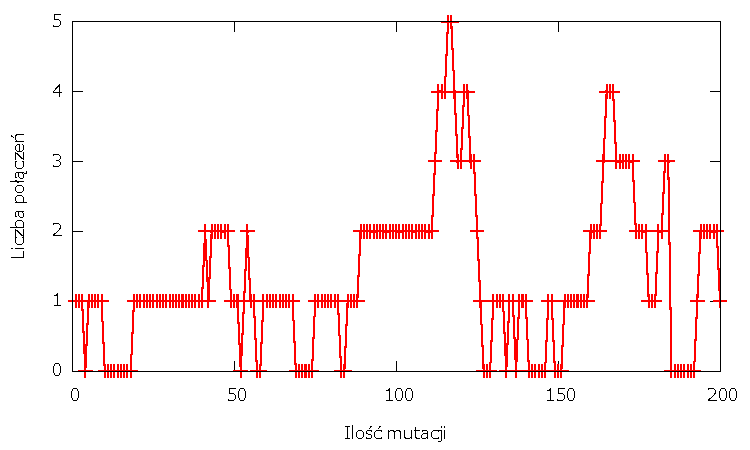
\includegraphics[width=0.8\textwidth]{dane/part2/zad2/connections}
	\caption{Ilości połączeń między neuronami w funkcji ilości mutacji.\label{fig:mutations-connections}}
	\end{figure}
		
	\end{itemize}
\item \textbf{Krzyżowanie}
	\begin{itemize}
		\item Wybierz jedną z reprezentacji: f0 lub f1.
		\item Stwórz dwie sieci neuronowe o tej samej topologii, różniące się tylko wagami.
		\item Dokonaj ich krzyżowania. Czy rezultat spełnia postulaty dobrego krzyżowania podane w poprzednim ćwiczeniu? 
		\\W konsoli:
				\begin{verbatim}
//cross over two neural networks.
//ensure there are two genotypes in the gene pool! 
GenePools.group=0; //select first group
GenePools.genotype=0; //select first genotype
GenePools.crossoverSelected(1); //cross over with the second genotype
Genotype.name="child"; //set descendant's name
GenePools.copySelected(0);
}
		\end{verbatim}
		\item Powtórz tę operację. Czy krzyżowanie jest deterministyczne?
		\item Powtórz to zadanie (krzyżowanie) dla pary sieci neuronowych o bardzo różnych topologiach.
	\end{itemize}
\end{enumerate}

%%%%%%%%%%%%%%%%%% Część III %%%%%%%%%%%%%%%%%

\section{Uczenie nienadzorowane warstwowych sieci neuronowych}

\subsection{Projektowanie i testowanie prostej sieci typu SOM}

\begin{enumerate}
\item \textbf{Utwórz sieć typu mapa odwzorowania cech istotnych (SOM) o wymiarach 5x4 (sugerowanych przez StatsticaNN) dla zbioru IRIS: File|New|Network, potem wybierz Kohonen, Advise, Create.}

\item \textbf{
Otwórz edytor sieci (Edit|Network). Jakiego typu neurony są stosowane w warstwie wyjściowej (okienko z ilustracją sieci to sugeruje) ?}

\item \textbf{
Zwróć uwagę, jak zdefiniowany jest błąd popełniany przez sieć (Error function) (Suma po wszystkich przykładach odległości pomiędzy przykładem a najbliższym mu wektorem wag neuronów w warstwie wyjściowej => uczenie nienadzorowane!)}

\item \textbf{
Zobacz, jak można zmieniać topologię sieci manewrując parametrem Width dla drugiej warstwy.}

\item \textbf{
Naucz sieć (Train|Kohonen) przy domyślnych ustawieniach parametrów. Zwróć uwagę, że mimo nienadzorowanego charakteru uczenia ma sens wyświetlanie przebiegu błędu.}

\item \textbf{
Co więcej, można używać zbioru weryfikującego i oprzeć na nim warunek stopu. Zbadaj, jak uczy się sieć np. z warunkiem stopu Minimum improvement|Verification = 0.01, Window = 10 (wydaje się to sensowne, bo widać, że minimum lokalne znajdowane jest bardzo szybko i nie ma potrzeby uczyć sieci aż przez 100 epok).}

\item \textbf{
Testowanie sieci. Obejrzyj najpierw, jak „odpowiadają” poszczególne neurony na kolejne przykłady ze zbioru uczącego (Run|Activations). Potem obejrzyj odpowiedzi sieci w diagramie, który zachowuje jej topologię (Run|Topological Map).  Jak grupują się przykłady ?
Zwróć uwagę, że podczas przeglądania przykładów mapą topologiczną, można samemu nazywać przykłady (górne pole bez nazwy) i/lub neurony (dolne pole bez nazwy); działa także prawy przycisk myszki.}

\item \textbf{
Poza tym można też obejrzeć statystykę „wygrywania” współzawodnictwa przez poszczególne neurony w poszczególnych podzbiorach (Statistics|Win frequencies).}

\item \textbf{
W podobny sposób naucz i przeanalizuj dla tego samego zbioru sieć o innej topologii (szczególnie ciekawe jest to dla sieci o topologii „jednowymiarowej”, gdzie warstwa wyjściowa ma np. 20 neuronów ułożonych w rzędzie, parametr Width = 1 dla warstwy 2 w edytorze sieci).}
	
\end{enumerate}

\subsection{ Analiza rzeczywistego problemu przy użyciu sieci SOM}

 \paragraph{\textbf{Dane: Zbiór PROTEIN.STA, dostępny lokalnie w katalogu Statistica (Examples). Opisuje on spożycie protein różnego pochodzenia w wybranych krajach Europy. Dane nie są podzielone na klasy decyzyjne.}}
 \paragraph{\textbf{Zbuduj sieć dla tego problemu (sugerowany rozmiar warstwy wyjściowej 4x4 lub nawet 3x3, bo mało przykładów). Naucz ją i przetestuj. Czy da się wyciągnąć i uzasadnić jakieś wnioski dotyczące podobieństwa poszczególnych krajów pod względem spożycia protein? Można, podobnie jak dla IRIS, spróbować z siecią SOM jednowymiarową.}}


\subsection{Projektowanie i testowanie prostej sieci typu SOM}
 \paragraph{\textbf{Zobacz, co się dzieje, gdy opcja "Shuffle cases" jest wyłączona. Sprawdź wpływ parametrów algorytmu uczącego (blisko "skrajnych" wartości parametrów) na przebieg i efekty uczenia.}}

%%%%%%%%%%%%%%%% literatura %%%%%%%%%%%%%%%%

%\bibliographystyle{plalpha}


\printbibliography
\end{document}

